\documentclass[10pt,twocolumn,letterpaper]{article}

\usepackage{cvpr}
\usepackage{times}
\usepackage{epsfig}
\usepackage{graphicx}
\usepackage{amsmath}
\usepackage{amssymb}

\newenvironment{myitemize}
{ \begin{itemize}
    \setlength{\itemsep}{0pt}
    \setlength{\parskip}{0pt}
    \setlength{\parsep}{0pt}     }
{ \end{itemize}                  }

% Include other packages here, before hyperref.

% If you comment hyperref and then uncomment it, you should delete
% egpaper.aux before re-running latex.  (Or just hit 'q' on the first latex
% run, let it finish, and you should be clear).
\usepackage[breaklinks=true,bookmarks=false]{hyperref}

\usepackage{subcaption}

\cvprfinalcopy % *** Uncomment this line for the final submission

% \def\cvprPaperID{****} % *** Enter the CVPR Paper ID here
\def\httilde{\mbox{\tt\raisebox{-.5ex}{\symbol{126}}}}

% Pages are numbered in submission mode, and unnumbered in camera-ready
\ifcvprfinal\pagestyle{empty}\fi
% \setcounter{page}{1}

%%%%%%%%% DEFINE COMMANDS HERE %%%%%%%%% 

\newcommand{\norm}[1]{\lVert #1 \rVert}

\begin{document}

%%%%%%%%% TITLE
\title{CS231N Project Milestone: Self-Supervised Feature Learning for Online Multi-Object Tracking}

\author{Bradley Collicott\\
Stanford University\\
{\tt\small collicott@stanford.edu}
\and
Mrunal Sarvaiya\\
Stanford University\\
{\tt\small mrunaljs@stanford.edu}
\and
Brian Weston\\
Stanford University\\
{\tt\small bweston@stanford.edu}
}

\maketitle

% Please make sure that all of the salient portions of the project have been addressed: 
% - Plan for using pre-trained networks / self-supervised learning. 
% - Using the DeepSORT framework
% - Comparing against the Cosine Metric Newtork as the Baseline

\begin{abstract}
The multi-object tracking problem has a rich history in both model-based on data-driven approaches. This project serves as an investigation into improving the performance of an online multi-object tracking pipeline by introducing a self-supervised feature extraction network to provide dense feature representations of detected pedestrians in video. Multiple pretext tasks for self-supervised representation learning will be explored and evaluated against a popular method from literature on the downstream task of multi-object tracking.
\end{abstract}

\section{Introduction}
% This section introduces your problem, and the overall plan for approaching your problem.
Multi-object tracking (MOT) from video lies at the intersection of multiple core problems in computer vision. Described in \cite{Ciaparrone2020}, the MOT process consists of 4 stages: Detection, Feature Extraction, Motion Prediction, and Data Association. As explored in the seminal work by Fortmann, Bar-Shalom, and Scheffé in 1980 \cite{Fortmann1980}, there is a rich history of using the model-based methods of joint probabilistic data association (JPDA) and multi-hypothesis tracking (MHT) to solve MOT. Only recently have the advances in deep learning permeated the field with impressive results. DeepSORT \cite{Wojke2018}, one of the current state-of-the-art methods in real-time tracking, uses deep learning to provide a dense feature representation for use in a data association algorithm. In contrast, other works have attempted an end-to-end deep learning approach to MOT using modern architectures like recurrent neural networks and transformers \cite{Bastani2021, Meinhardt2021}. These methods prove effective but suffer high training time, computation, and memory costs.

The data association step (i.e. associating a detection with an existing trajectory) in MOT is widely considered to be the bottleneck for current performance. Therefore, this work seeks to investigate methods for improving feature representation to reduce the likelihood of ID switching (IDSW) and incorrect associations. Recent works have shown that self-supervised learning \cite{Jing2021} can imbue networks with the ability to learn context and salient features by solving a non-trivial pretext task at training time. The selection of pretext task depends on the downstream application, but in all cases the solution to the task is self-evident from the input, e.g. ordering a set of unordered video frames. Gidaris et al. \cite{Gidaris2019} demonstrated that few-shot learning could be improved by fine-tuning a pre-trained feature extraction network using self-supervised representation learning. With this in mind, the effectiveness of fine-tuning a pre-trained feature extraction network with multiple pretext tasks will be investigated for improving MOT performance.

\section{Problem Statement}
% Describe your problem precisely specifying the dataset to be used, expected results and evaluation.
The multi-object tracking problem can be decomposed into detection, feature extraction, motion prediction, and data association steps. The general multi-object tracking problem formulation, datasets, and methods of evaluation are discussed here.
\subsection{Multi-Object Tracking}
The objective of MOT is to detect the objects of interest and track them across multiple time steps. In the tracking-by-detection paradigm, this includes extracting the features of each detection and comparing with previously extracted features to associate each detection with the correct ID -- in this way, MOT is largely a data association problem. Further, online MOT addresses the problem of tracking objects in real-time by sequentially processing video frames.
\subsection{Datasets}
The primary training and evaluation dataset will be the MOT17 \cite{MOT17} pedestrian tracking dataset. This dataset provides pedestrian detections from a Faster-RCNN network with ground truth annotations for over 1300 unique IDs across over 11,000 frames. A sample frame from the MOT17 training data is shown in Figure 1.
\begin{figure}[h!]
    \centering
    \begin{subfigure}[b]{0.48\linewidth}
        \centering
        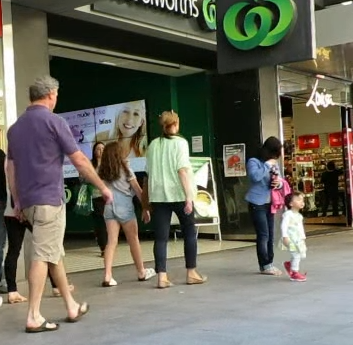
\includegraphics[width=\linewidth]{docs/milestone/figs/MOT17_raw.png}
        \caption{Raw}
        \label{fig:my_label}
    \end{subfigure}
    \hfill
    \begin{subfigure}[b]{0.48\linewidth}
        \centering
        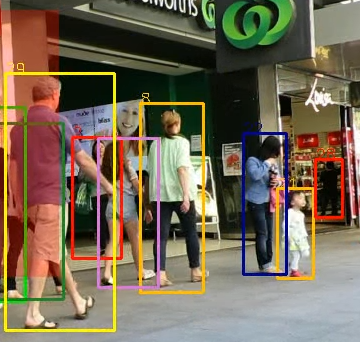
\includegraphics[width=\linewidth]{docs/milestone/figs/MOT17_gt.png}
        \caption{Annotated}
        \label{fig:my_label}
    \end{subfigure}
    \caption{MOT17 Sample Scene}
\end{figure}
\subsection{Metrics and Evaluation}
The CLEAR MOT metrics established in \cite{Bernardin2008} will be used to evaluate tracking performance. We define the following terms for computing metrics:
\begin{myitemize}
    \item False Negative: Ground truth bounding box that cannot be associated with a hypothesis
    \item False Positive: Hypothesis that cannot be associated with a ground truth bounding box
    \item ID Switch: A change to a correct ground truth ID association
\end{myitemize}
The catch-all metric for tracking is the multi-object tracking accuracy (MOTA).
\begin{equation}
    MOTA = 1-\frac{FN+FP+IDSW}{GT}  \in (-\infty, 1]
\end{equation}
Where $FN$, $FP$, $IDSW$, and $GT$ are the number of false positives, false negatives, ID switches, and ground truth tracks across all frames, respectively. 

In addition to the CLEAR MOT metrics, it is common to use the Mostly Tracked (MT) and Mostly Lost (ML) metrics to capture the number of trajectories correctly and incorrectly tracked for at least $80\%$ of the frames in which the tracks are present. Since this project will use public detections, the ML, MT, and IDSW metrics will be most informative for assessing performance.
\section{Technical Approach}
% Describe the methods you intend to apply to solve the given problem
To limit the scope of this project to self-supervised learning, the Deep SORT MOT pipeline \cite{Wojke2018} will be adopted as the motion prediction and data association backend. Likewise, the public detections available with MOT datasets will be used to allow for explicit comparison of the effectiveness between feature extraction networks rather than conflating with detector performance. 
% \subsection{Multi-Object Tracking Architecture}
% thinking about skipping details here to focus more on the pretext tasks, our choice of networks, and metrics/task evaluation
\subsection{Pretext Tasks}
Pretext tasks are used in self-supervised learning to encourage neural networks to learn a representation that is useful for a separate downstream task. Three pretext tasks were selected to learn representations for evaluation on the downstream application of MOT.
\subsubsection{Predicting Future Video Frames}
% I plan on writing a short problem formulation, proposed network to solve the problem, Loss metrics, and plans for generating labels for my pretext task.

To learn spatial and temporal context from single video frames, a pretext task of predicting sequential video frames will be introduced. Given a bounding box image patch as an input, a network will be tasked with predicting the next bounding box image crop corresponding to the same pedestrian. 

Using the pre-trained network from the DeepSORT paper as an encoder network and re-initializing the final two convolutional layers, a decoder CNN will be affixed to the end of the network to support decoding the feature vector into a predicted RGB image.
The loss for each image can be computed as the reconstruction loss between the predicted image $\hat{I}$ and the true next image $I$ in the video sequence.
\begin{equation}
    \mathcal{L} = \sum_{i=1}^N \norm{I_i-\hat{I}_i}_2^2
\end{equation}
The dense feature representation learned at the end of the encoder network will be used in the downstream MOT task for person re-identification. By learning to predict the next bounding box image, the network will require an understanding of the foreground/background separation, leading to better feature representation for the person in the image.
\subsubsection{Predicting Image Rotations}
One of the pretext tasks considered is predicting image rotations. The goal of this network is to learn features that enable it predict the correct 2D rotation that is applied to the image as an input. We start with the pretrained network used as the feature extractor in DeepSORT. We replace the last two layers (Batch and l2 normalization and Dense 10) with two fully connected layers as done in the original RotNet model \cite{Johnson20}. Finally, the loss function is the same as the one used in \cite{gidaris2018unsupervised} which is the negative log likelihood of the data set.


The model will be trained in a self supervised way using the cropped detection bound boxes from the MOT17 dataset. Since the model will learn to predict the correct rotations of humans, we expect the learned features to be useful in similar tasks, which in this case would be the affinity computation stage in the MOT tracking framework. 

\subsubsection{Predicting Color in Video Frames}
The final pretext task considered is colorization. The goal of the network is to learn embeddings to correctly predict the color in images from gray-scale version of the image. Starting again with the pretrained network as the inital feature extractor in DeepSORT, we strip the last two layers and the fine-tune new layers using this new self-supervised pretext task. 

The model will be trained in a self-supervised way where we take the cropped detection bounding boxes from the MOT17 dataset. After the model is trained to learn color of the humans, clothes, and background, we expect the model to learn to track visual features and assist with data association problem \cite{Vondrick_2018_ECCV}.



\subsection{Baseline}
The baseline method will be a network trained using the deep cosine metric \cite{Wojke2018cosine} from the original DeepSORT feature extractor. Consideration will be given to model size and parameter counts to ensure fair comparison between methods.
\section{Preliminary Results}
% State and evaluate your results up to the milestone
At this stage, a code framework has been developed for training a neural network in using PyTorch. The framework has been tested on a representative network using a simple classification task.

Pretext tasks and pre-trained network architectures have been selected for use, and immediate next steps include creating the architecture for self-supervised learning, generating ground truth labels for pretext tasks, and visualizing training results.

{\small
\bibliographystyle{ieee}
\bibliography{references}
}

\end{document}
